\documentclass[12pt, times new roman, a4paper]{article}
\linespread{1,5}
\usepackage[utf8]{inputenc}
\usepackage{graphicx}
\renewcommand{\figurename}{Gambar}

\begin{document}

\section{TEORI}

\subsection{Sejarah Python dan Perbedaan python 2 dan 3}

\subsubsection{Sejarah Python}

Python dikembangkan oleh Guido van Rossum di Stichting Mathematisch Centrum (CWI) pada tahun 1990, Amsterdam sebagai terusan dari bahasa pemrograman ABC. Versi penutup yang diluncurkan Stichting Mathematisch Centrum (CWI) adalah 1.2.

Guido pindah ke CNRI di Virginia Amerika dengan tetap meneruskan pengembangan Python pada tahun 1995. Versi penutup yang diluncurkan adalah 1.6. Guido dan para pengembang pokok Python pindah ke BeOpen.com yang merupakan sebuah perusahaan komersial dan membentuk BeOpen PythonLabs pada tahun 2000. Python 2.0 diluncurkankan oleh BeOpen. Sesudah meluncurkan Python 2.0, Guido dan beberapa anggota tim PythonLabs pindah ke DigitalCreations.

Pada saat ini pengembangan Python tetap dilakukan oleh sejumlah pemrogram yang dikomandoi oleh Guido dan Python Software Foundation. Python Software Foundation ialah suatu perserikatan non-penghasilan yang dibuat sebagai pemilik hak cipta cendikiawan Python sedari versi 2.1 dan dengan demikian mencegah Python dimiliki oleh perusahaan komersial. Pada saat ini penyebaran Python telah mencapai versi 2.7.14 dan versi 3.6.3.\\

\subsubsection{Perbedaan python 2 dan 3}

\subsubsection*{1. untuk mencetak teks atau yang lainnya}
Python 2\\
perintah :\\
print “Gak gunakan kurung bisa”\\
print(“gunakan kurung juga bisa”)\\
Print “ini”, ; print “untuk cetak satu baris aja”\\
Python 3\\
perintah :\\
print(“wajib gunakan kurung”)\\
print (“ini digunakan untuk “, end=””)\\
print (“untuk cetak satu baris”)

\subsubsection*{2. Syntax untuk meminta inputan}
Python 2\\
perintah :\\
kelas = raw\textunderscore input(‘kelas anda : ‘)\\
print kelas\\
Python 3\\
perintah\\
kelas = input(“kelas anda : “)\\
print (kelas)

\subsubsection*{3. Hasil dari operator pembagian}
Python 2\\
perintah :\\
print "3 / 2 = " , 3/2\\
print "3 // 2 = " , 3//2\\
print "3 / 2.0 = " , 3/2.0\\
print "3 // 2.0 = " , 3//2.0\\
Python 3\\
perintah :\\
print ("3 / 2 = " , 3/2)\\
print ("3 // 2 = " , 3//2)\\
print ("3 / 2.0 = " , 3/2.0)\\
print ("3 // 2.0 = " , 3//2.0)\\

\subsubsection*{4. Implementasi dan penggunaan Python di perusahaan dunia}

\subsubsection*{A. Spotify}
Sistem rekomendasi Spotify bergantung pada analisis data yang sangat besar, untuk menginterpretasikan analisis tersebut Spotify menggunakan Luigi, modul Python yang sinkron dengan Hadoop. Modul open source ini menangani satu library dengan library lainnya agar saling bekerjasama, dan mengkonsolidasi eror log secara cepat.

\subsubsection*{B. Google}
Dari awal berdiri, Google sudah menggunakan Python, bahkan Python merupakan salah satu bahasa pemrograman yang penting bagi Google, itulah mengapa Google pernah merekrut kreator Python Guido Van Rossum untuk bekerja di Google, alasannya adalah karena kemudahan dalam perawatan.

\subsubsection*{C. Industrial Light and Magic}
Menggunakan Python, ILM dapat dengan mudah membungkus komponen software dan meningkatkan aplikasi grafis mereka. Hingga saat ini ILM tetap menggunakan Python karena selalu dapat menghadirkan solusi terbaik untuk kebutuhan mereka.

\subsubsection*{D. Netflix}
Salah satu penggunaan utama Python di aplikasi Netflix adalah pada Central Alert Gateway. Aplikasi RESTful ini akan me-reroute alert dan mengirimkannya pada kelompok atau individu yang berhak melihatnya. Sebagai tambahan aplikasi ini akan secara otomatis reboot atau menghentikan proses yang dianggap bermasalah. Selain C.A.G, Python juga digunakan pada aplikasi untuk menelusuri riwayat dan perubahan pengaturan keamanan.

\subsubsection*{E. Instagram}
Seperti yang kita ketahui, Instagram telah merevolusi komunikasi visual dan pemasaran digital melalui media foto. Dengan 400 juta pengguna aktif setiap harinya, tentu ini menghapus pendapat yang mengatakan bahwa aplikasi python tidak terlalu scalable. Menurut Hui Ding, engineer di Instagram, moto para pengembang aplikasi di instagram adalah “Do the simple thing first,” dan hal ini sangat bisa dilakukan menggunakan Python, bagi para pengembang aplikasi di Instagram Python sangat ramah pengguna, sederhana dan rapi. Juga karena Python sangat populer, maka tidaklah sulit menemukan pengembang baru untuk memperbesar tim.\\
Selain perusahaan diatas ada beberapa perusahaan pengguna Python lain yang layak untuk disebutkan\\
-Pinterest\\
-Disqus\\
-Dropbox\\
-Uber\\
-Reddit\\
-Quora\\
-Facebook (Bahasa ke-3 setelah PHP (Hack) dan C++, digunakan untuk manajemen infrastruktur)\\

\section{INSTALASI}

\subsection{Instalasi Pyhton 3}

\subsubsection{Klik Instal Now}
	\begin{figure}[h]
		\centering
		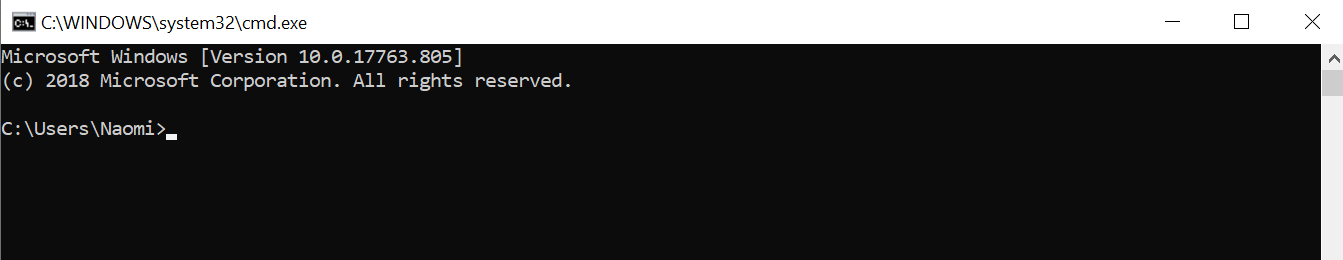
\includegraphics[scale=0.7]{Gambar/p1}
		\caption{Instal Pyhton 3.8.0}
	\end{figure}
\subsubsection{Tunggu hingga proses selesai}
	\begin{figure}[h]
		\centering
		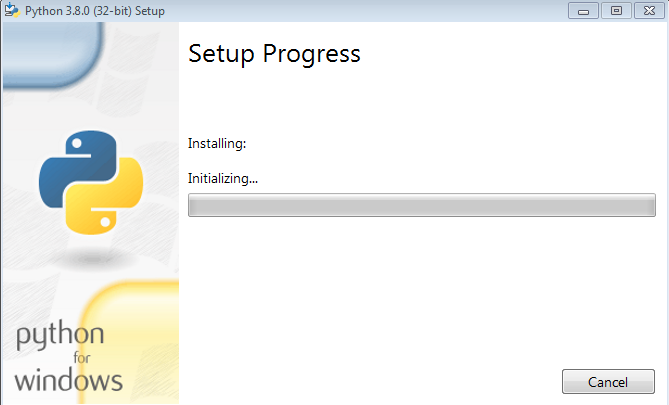
\includegraphics[scale=0.55]{Gambar/p2}
		\caption{Instal Pyhton 3.8.0}
	\end{figure}
\subsubsection{Selesai klik close}
	\begin{figure}[h]
		\centering
		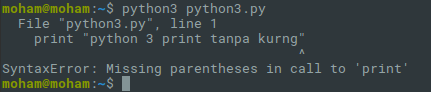
\includegraphics[scale=0.55]{Gambar/p3}
		\caption{Instal Pyhton 3.8.0}
	\end{figure}

\subsection{Instalasi pip}

\subsubsection{Pastikan file pip yang telah anda download diletakkan di desktop}
\subsubsection{ketik kode cd desktop pada CMD}
\subsubsection{Setelah itu ketik python get-pip.py}
	
	\begin{figure}[h]
		\centering
		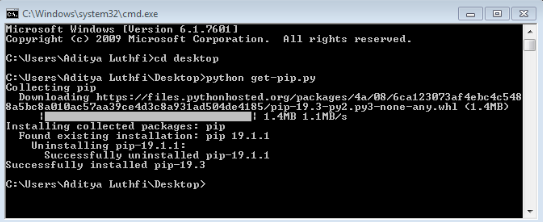
\includegraphics[scale=0.6]{Gambar/y}
		\caption{Instal pip 3.8.0}
	\end{figure}
	
\subsection{Setting environment}
	
\subsection{entrepreter/cli melalui terminal}
\subsubsection{ketik kode python pada terminal}
\subsubsection{kelas = input(“kelas anda : “)}
	\begin{figure}[h]
		\centering
		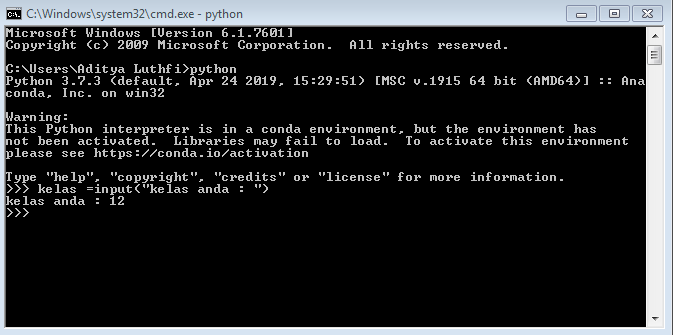
\includegraphics[scale=0.4]{Gambar/e}
		\caption{entrepreter melalui terminal}
	\end{figure}
	
\subsection{Menjalankan dan mengupdate annaconda dan spyder}
	
\subsubsection{Buka CMD dan ketik install -c annaconda python}
	\begin{figure}[h]
		\centering
		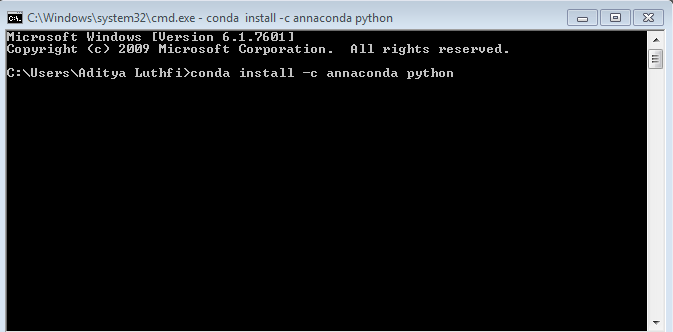
\includegraphics[scale=0.3]{Gambar/c1}
		\caption{Update annaconda}
	\end{figure}
\subsubsection{tekan y untuk melanjutkan update}
	\begin{figure}[h]
		\centering
		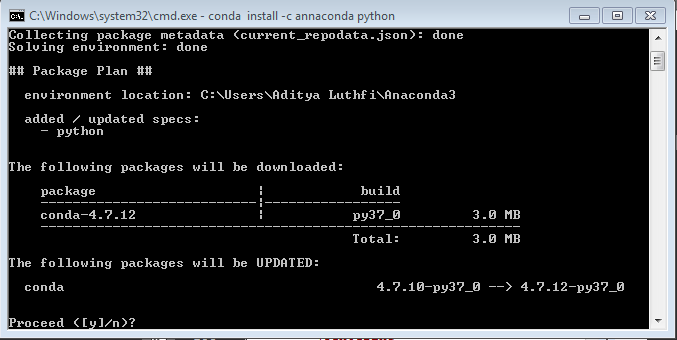
\includegraphics[scale=0.3]{Gambar/c2}
		\caption{Update annaconda}
	\end{figure}
\subsubsection{Buka Spyder untuk mengecek versi}
	\begin{figure}[h]
		\centering
		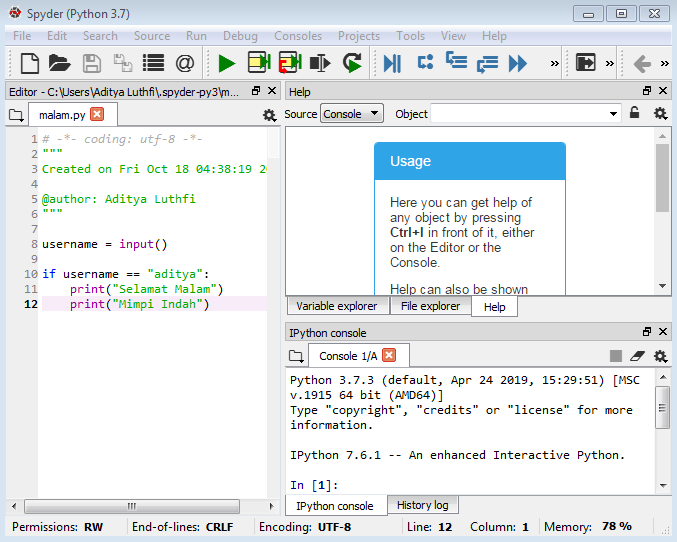
\includegraphics[scale=0.2]{Gambar/c3}
		\caption{Update annaconda}
	\end{figure}	
	
\subsection{Menjalankan Script hello word di spyder}

\subsubsection{ketik print ("Hello World")}
	\begin{figure}[h]
		\centering
		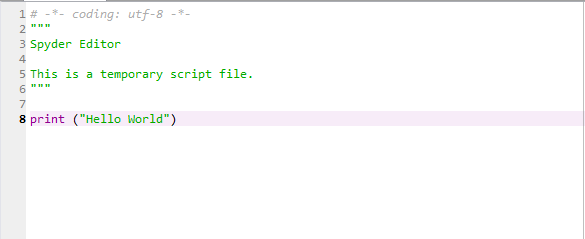
\includegraphics[scale=0.7]{Gambar/h1}
		\caption{Script hello word}
	\end{figure}
\subsubsection{Run file akan mencetak Hello World pada console}
	\begin{figure}[h]
		\centering
		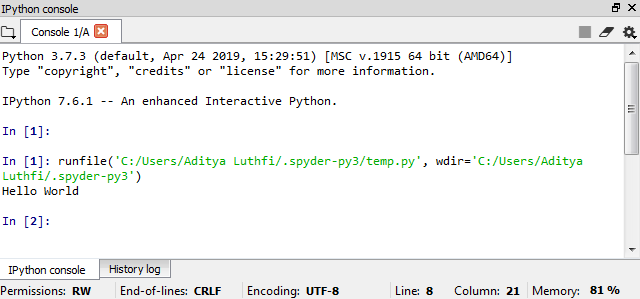
\includegraphics[scale=0.7]{Gambar/h2}
		\caption{Script hello word}
	\end{figure}
	
\subsection{Otomatis Login di siap.poltekpos}

\subsection{Pemakaian Variabel Explorer}
Variable explorer akan terbentuk secara otomatis ketika membuat suatu variable, pada variable explorer kita bisa melihat nama variable, tipe data, size dari variable tersebut.
	\begin{figure}[h]
		\centering
		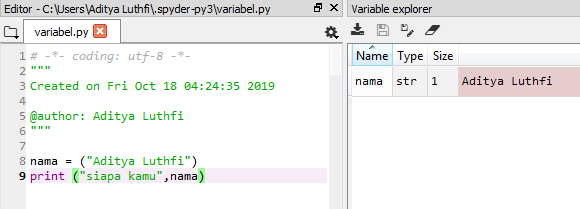
\includegraphics[scale=0.5]{Gambar/v}
		\caption{Script hello word}
	\end{figure}
	
\section{Identasi}
Identasi merupakan bagian dari suatu paragraf yang menjorok kedalam pada baris tiap paragraf. Mengatur indentasi dengan cara menggunakan tab atau spasi. Identasi digunakan oleh bahasa pemrograman python sebagai pengganti briket ({}) untuk membuka dan menutup suatu fungsi. Error indentasi dapat terjadi jika syntax tidak menggunakan tab atau space.

\subsection{Jenis-Jenis Error Indentasi}
	\begin{figure}[h]
		\centering
		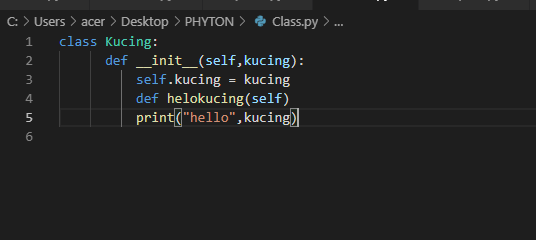
\includegraphics[scale=0.7]{Gambar/a}
		\caption{Indentasi}
	\end{figure}
Jika di run maka error seperti ini. 
	\begin{figure}[h]
		\centering
		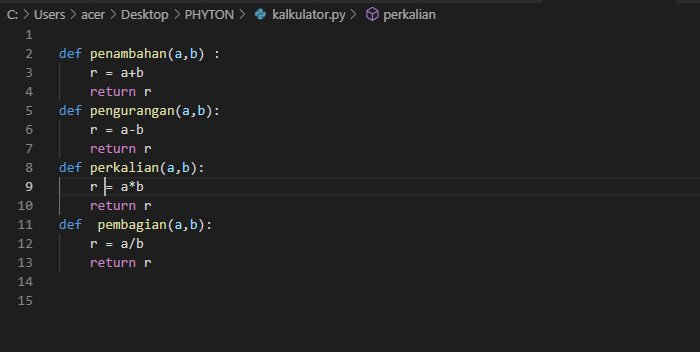
\includegraphics[scale=0.9]{Gambar/b}
		\caption{Error Indentasi}
	\end{figure}

\subsection{Cara Menangatasi Error}
Mengatasi error indentasi bisa diatasi dengan menambahkan tab atau space pada line atau baris yang terdapat error.

\begin{figure}[h]
		\centering
		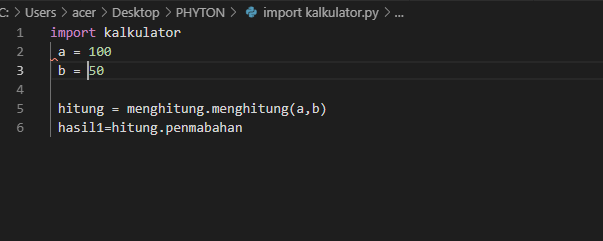
\includegraphics[scale=1]{Gambar/c}
		\caption{Error yang sudah ditangani}
	\end{figure}

\end{document}
